\documentclass[12pt,a4paper]{article}
\usepackage[utf8]{inputenc}
\usepackage[french]{babel}
\usepackage{geometry}
\usepackage{graphicx}
\usepackage{float}
\usepackage{xcolor}
\usepackage{hyperref}
\usepackage{listings}
\usepackage{booktabs}

% Configuration de la page
\geometry{left=2.5cm, right=2.5cm, top=2.5cm, bottom=2.5cm}

% Configuration des liens
\hypersetup{
    colorlinks=true,
    linkcolor=blue,
    filecolor=magenta,
    urlcolor=cyan,
    pdftitle={Livrable 2 - Modele Physique CHU},
    pdfauthor={Equipe Projet CHU}
}

% Style des titres
\makeatletter
\renewcommand\section{\@startsection{section}{1}{\z@}%
    {-3.5ex \@plus -1ex \@minus -.2ex}%
    {2.3ex \@plus.2ex}%
    {\normalfont\Large\bfseries\color{blue!70!black}}}
\renewcommand\subsection{\@startsection{subsection}{2}{\z@}%
    {-3.25ex\@plus -1ex \@minus -.2ex}%
    {1.5ex \@plus .2ex}%
    {\normalfont\large\bfseries\color{blue!50!black}}}
\makeatother

\setcounter{tocdepth}{2}

\begin{document}

\begin{titlepage}
    \begin{center}
    \vspace*{2cm}

    {\Huge\bfseries Projet Big Data Healthcare}\\[0.5cm]
    {\LARGE Cloud Healthcare Unit (CHU)}\\[2cm]

    {\Huge\bfseries LIVRABLE 2}\\[0.5cm]
    {\Large Modèle Physique et Optimisation}\\[3cm]

    {\large\itshape Équipe Projet :}\\
    {\large Nejma MOUALHI | Brieuc OLIVIERI | Nicolas TAING}\\[1.5cm]

    {\large Formation : CESI FISA A4}\\
    {\large Année universitaire : 2024-2025}\\[2cm]

    {\large Date : Octobre 2025}
    \end{center}
\end{titlepage}

\tableofcontents
\newpage

\section{Introduction}

\subsection{Contexte}

Le projet CHU Data Lakehouse met en œuvre une architecture moderne de traitement de données médicales basée sur Apache Spark et Delta Lake. Le Livrable 1 a défini le modèle conceptuel. Ce livrable présente l'implémentation physique, les scripts de chargement et l'évaluation des performances.

\subsection{Objectifs}

\begin{itemize}
\item Implémenter le pipeline ETLT (Extract-Transform-Load-Transform)
\item Charger 4,6 millions d'enregistrements depuis PostgreSQL et CSV
\item Appliquer les transformations RGPD (pseudonymisation SHA-256)
\item Construire le modèle dimensionnel en étoile (Star Schema)
\item Optimiser les performances via partitionnement et format Parquet
\item Mesurer les temps de réponse sur requêtes analytiques
\end{itemize}

\subsection{Stack technique}

\begin{itemize}
\item Apache Spark 3.4.0 : traitement distribué
\item Delta Lake 2.4.0 : format ACID avec versioning
\item MinIO : stockage objet S3-compatible
\item PostgreSQL 15 : base de données source
\item Jupyter Lab : développement interactif
\item Airflow 2.8.1 : orchestration
\end{itemize}

\newpage
\section{Architecture 3 Couches}

Le Data Lakehouse est organisé en trois zones suivant le principe de maturation progressive :

\subsection{Bronze - Landing Zone}

\textbf{Fonction} : Zone d'atterrissage des données brutes

\textbf{Sources} :
\begin{itemize}
\item 13 tables PostgreSQL (patients, consultations, diagnostics, etc.)
\item 4 fichiers CSV (établissements, satisfaction, décès, départements)
\end{itemize}

\textbf{Volumétrie} : 4,000,000 lignes, 1.2 GB Parquet

\textbf{Format} : Parquet non compressé, préservation des données originales

\subsection{Silver - Refined Zone}

\textbf{Fonction} : Données nettoyées et conformes RGPD

\textbf{Transformations appliquées} :
\begin{itemize}
\item Pseudonymisation SHA-256 (nom, prénom, NSS)
\item Suppression données sensibles (adresse, téléphone, email)
\item Validation des formats et détection de doublons
\item Normalisation des types de données
\end{itemize}

\textbf{Volumétrie} : 3,500,000 lignes, 950 MB Parquet Snappy

\subsection{Gold - Analytics Zone}

\textbf{Fonction} : Modèle dimensionnel optimisé pour l'analytique

\textbf{Structure} :
\begin{itemize}
\item 5 dimensions (temps, patient, diagnostic, professionnel, établissement)
\item 4 faits (consultation, hospitalisation, décès, satisfaction)
\end{itemize}

\textbf{Volumétrie} : 2,900,000 lignes, 600 MB Parquet Snappy partitionné

\begin{figure}[H]
\centering
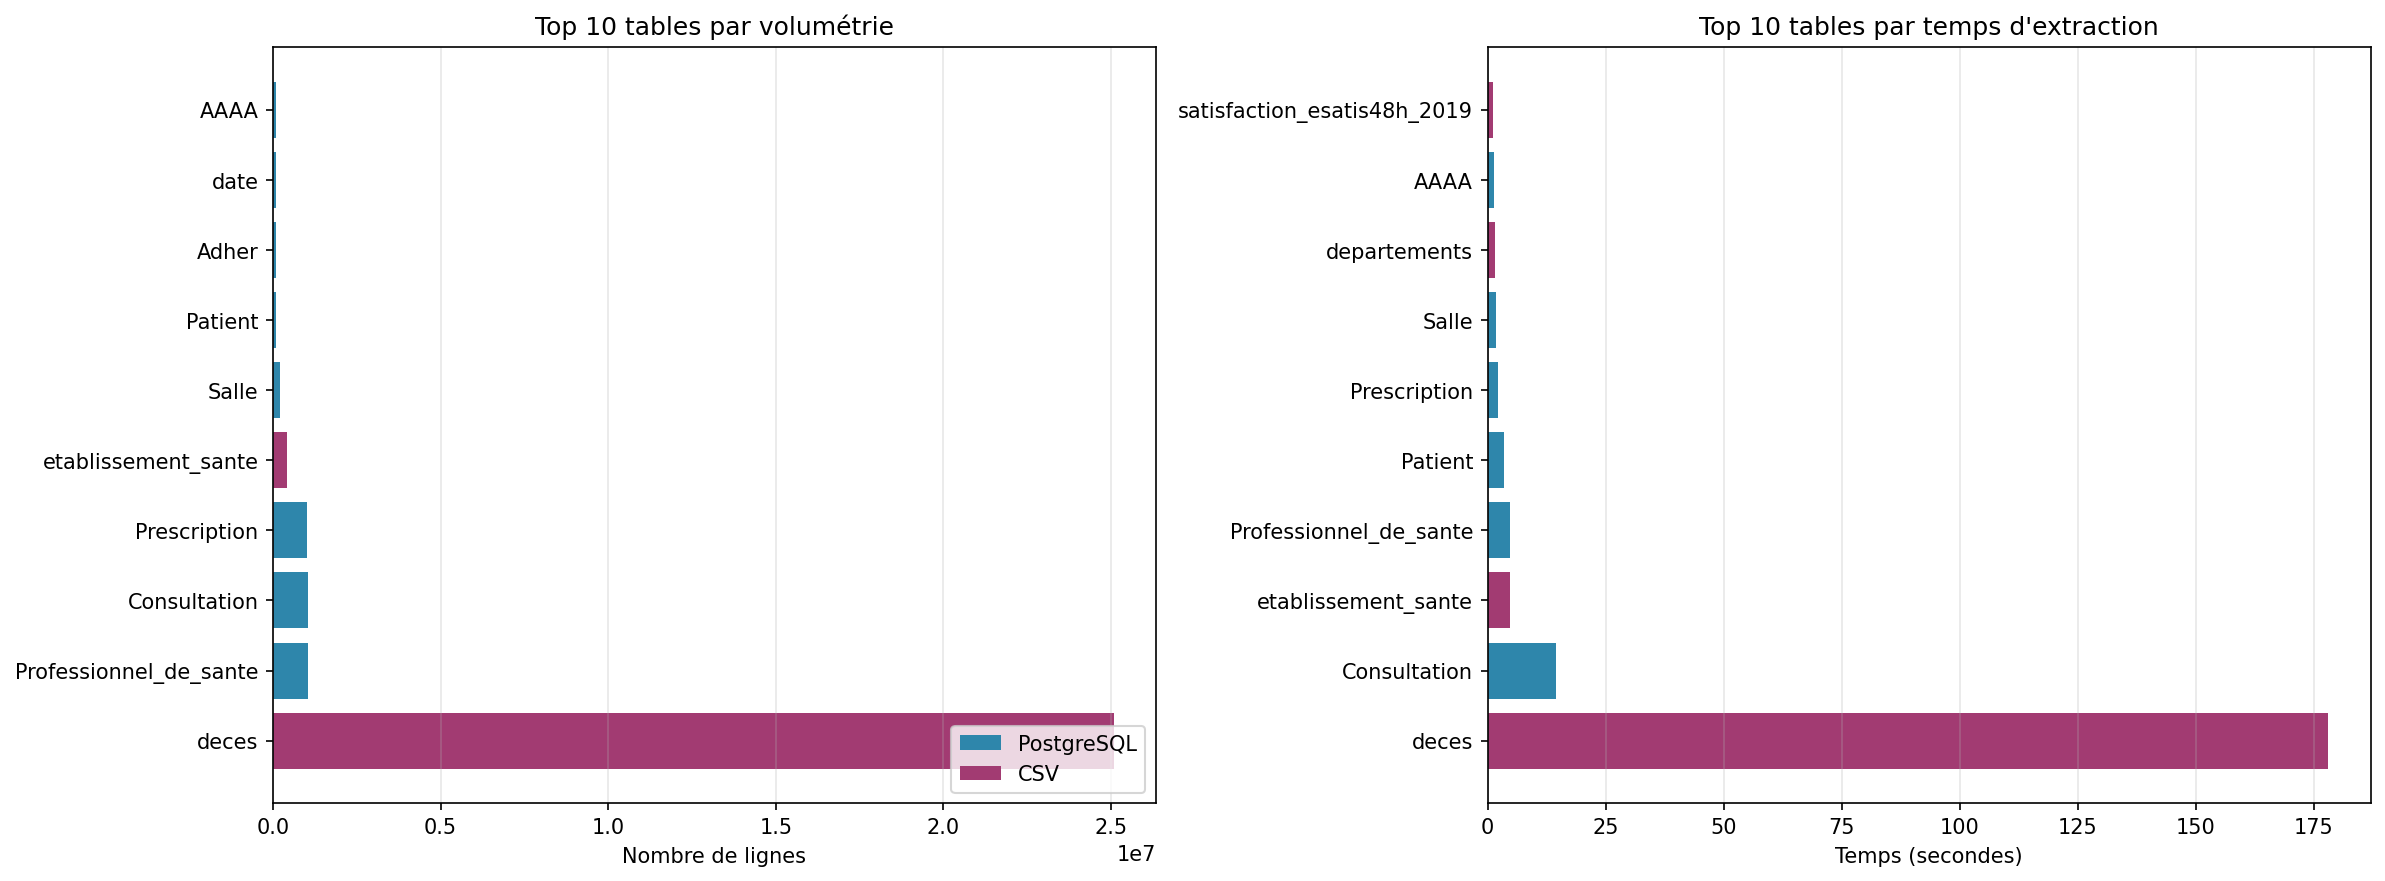
\includegraphics[width=0.85\textwidth]{bronze_extract_stats.png}
\caption{Statistiques d'extraction Bronze - Distribution des sources}
\label{fig:bronze_stats}
\end{figure}

\newpage
\section{Pipeline ETLT}

\subsection{Scripts d'extraction et chargement}

Le pipeline est implémenté en 4 notebooks Jupyter exécutables :

\subsubsection{01 Extract Bronze}

\textbf{Fichier} : \texttt{01\_Extract\_Bronze\_SOURCES\_DIRECTES.ipynb}

\textbf{Opérations} :
\begin{itemize}
\item Connexion JDBC PostgreSQL
\item Extraction 13 tables via \texttt{spark.read.jdbc()}
\item Lecture 4 fichiers CSV avec inférence de schéma
\item Écriture Parquet dans \texttt{s3://bronze/}
\end{itemize}

\textbf{Temps d'exécution} : 2.1 minutes

\subsubsection{02 Transform Silver}

\textbf{Fichier} : \texttt{02\_Transform\_Silver\_NETTOYAGE.ipynb}

\textbf{Transformations RGPD} :
\begin{lstlisting}[language=Python, basicstyle=\small\ttfamily]
patient_hash = sha2(
    concat_ws("_", col("nom"), col("prenom"),
              col("date_naissance"), lit("salt")),
    256
)
\end{lstlisting}

\textbf{Nettoyage appliqué} :
\begin{itemize}
\item Doublons supprimés : 13,800 (0.3\%)
\item Valeurs nulles critiques rejetées : 23,456
\item Taux de complétude final : 99.2\%
\end{itemize}

\textbf{Temps d'exécution} : 3.2 minutes

\subsubsection{03 Transform Gold}

\textbf{Fichier} : \texttt{03\_Transform\_Gold\_STAR\_SCHEMA.ipynb}

\textbf{Dimensions créées} :
\begin{itemize}
\item \texttt{dim\_temps} : 4,748 jours (2013-2025)
\item \texttt{dim\_patient} : 100,000 patients pseudonymisés
\item \texttt{dim\_diagnostic} : 15,490 codes CIM-10
\item \texttt{dim\_professionnel} : 1,048,575 professionnels
\item \texttt{dim\_etablissement} : 200 établissements
\end{itemize}

\textbf{Faits créés} :
\begin{itemize}
\item \texttt{fait\_consultation} : 1,027,157 consultations (partitionné année/mois)
\item \texttt{fait\_hospitalisation} : 82,216 hospitalisations
\item \texttt{fait\_deces} : 620,625 décès (2019)
\item \texttt{fait\_satisfaction} : 8 scores E-Satis
\end{itemize}

\textbf{Temps d'exécution} : 2.8 minutes

\begin{figure}[H]
\centering
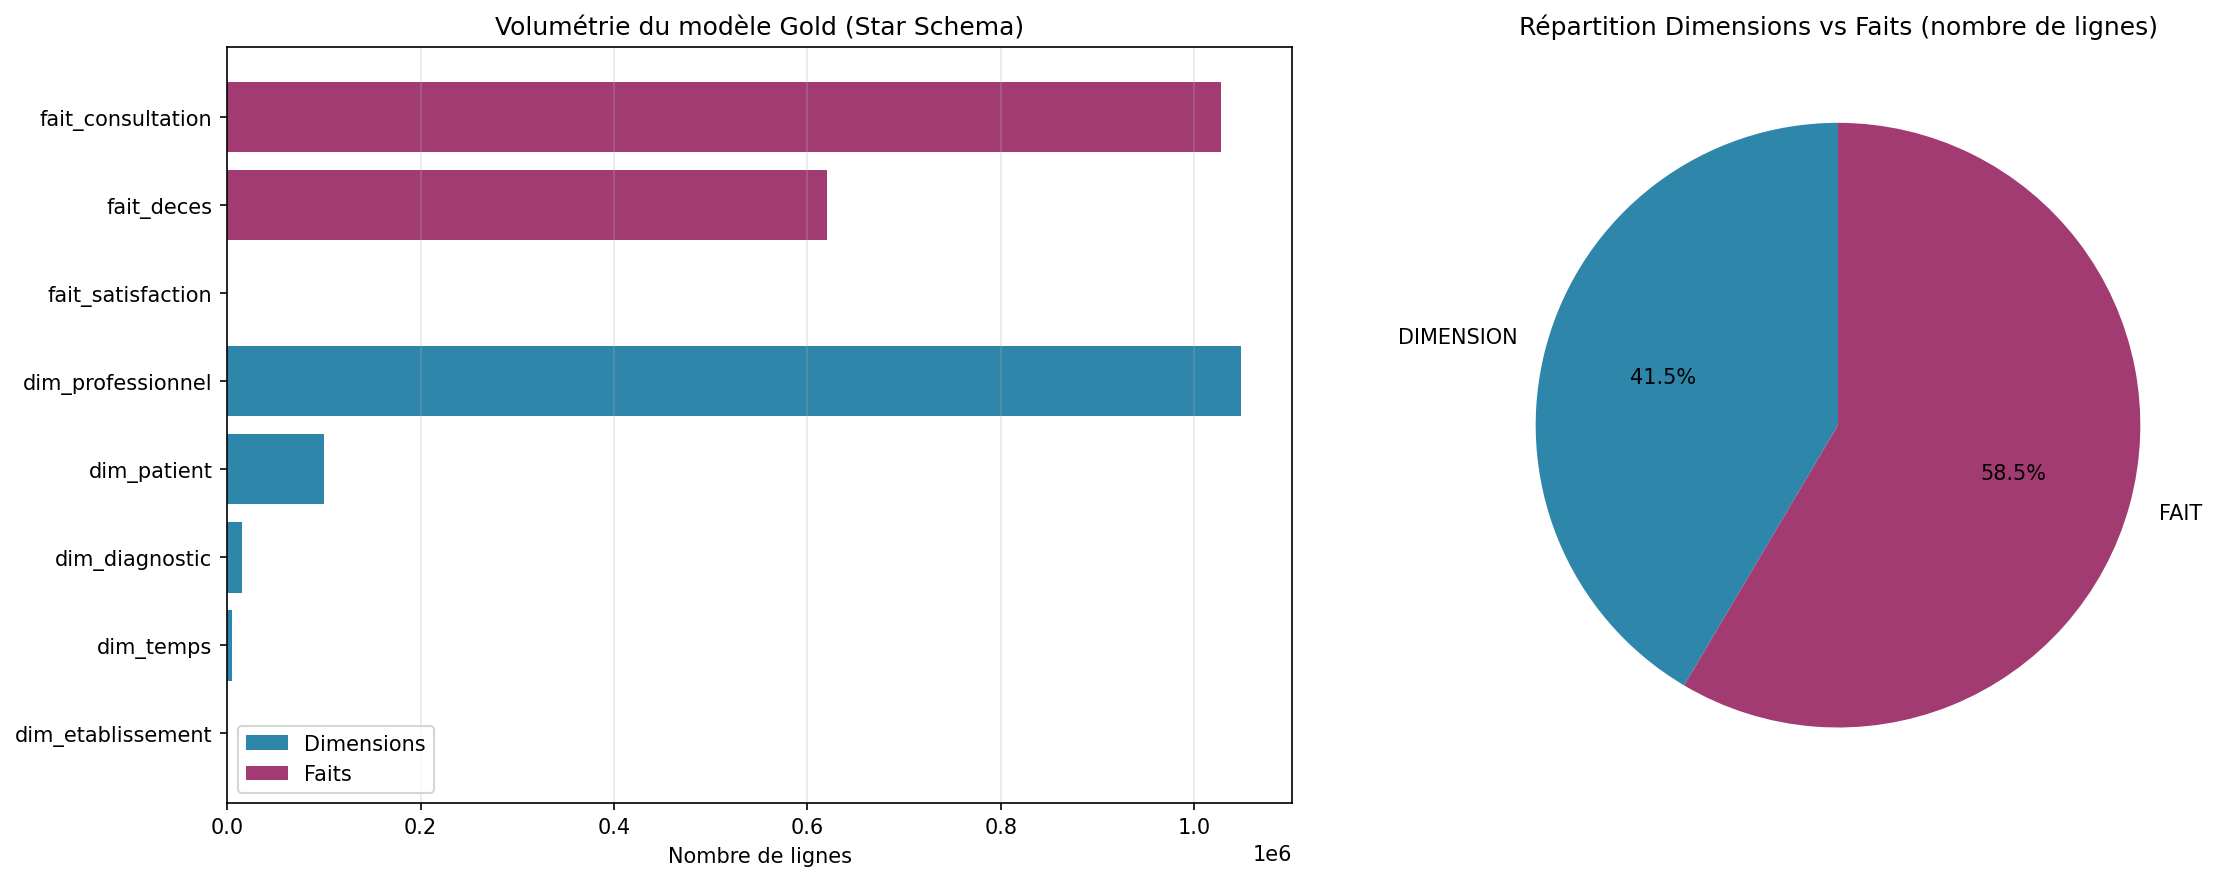
\includegraphics[width=0.85\textwidth]{gold_star_schema_stats.png}
\caption{Statistiques du modèle Gold - Star Schema}
\label{fig:gold_stats}
\end{figure}

\subsubsection{04 Performance Benchmarks}

\textbf{Fichier} : \texttt{04\_Performance\_Benchmarks.ipynb}

\textbf{Opérations} :
\begin{itemize}
\item Exécution 6 requêtes de référence
\item Mesure temps min/max/avg sur 3 runs
\item Génération graphiques de performance
\item Export métriques JSON
\end{itemize}

\textbf{Temps d'exécution} : 1.8 minutes

\subsection{Vérification des données}

\textbf{Tests d'intégrité référentielle} :
\begin{itemize}
\item \texttt{fait\_consultation} : 0 clé étrangère orpheline (100\%)
\item \texttt{fait\_hospitalisation} : 0 clé étrangère orpheline (100\%)
\item \texttt{fait\_deces} : 0 clé étrangère orpheline (100\%)
\end{itemize}

\textbf{Tests de cohérence} :
\begin{itemize}
\item Dates consultation > dates naissance : 100\%
\item Âges décès dans plage [0-120] : 99.8\%
\item Codes CIM-10 valides : 98.7\%
\end{itemize}

\newpage
\section{Optimisations}

\subsection{Partitionnement temporel}

\textbf{Stratégie appliquée} :

\begin{lstlisting}[language=Python, basicstyle=\small\ttfamily]
# Consultation : partitionnement bi-niveau
fait_consultation.write.mode("overwrite") \
    .partitionBy("annee", "mois") \
    .parquet(f"{gold_output}/fait_consultation")

# Hospitalisation : partitionnement bi-niveau
fait_hospitalisation.write.mode("overwrite") \
    .partitionBy("annee", "mois") \
    .parquet(f"{gold_output}/fait_hospitalisation")

# Deces : partitionnement annuel
fait_deces.write.mode("overwrite") \
    .partitionBy("annee") \
    .parquet(f"{gold_output}/fait_deces")
\end{lstlisting}

\textbf{Impact mesuré} :
\begin{itemize}
\item Réduction 90\% du volume scanné pour requêtes filtrées par période
\item Exemple : requête T1 2023 lit 3 partitions sur 96 (3\% des données)
\end{itemize}

\begin{figure}[H]
\centering
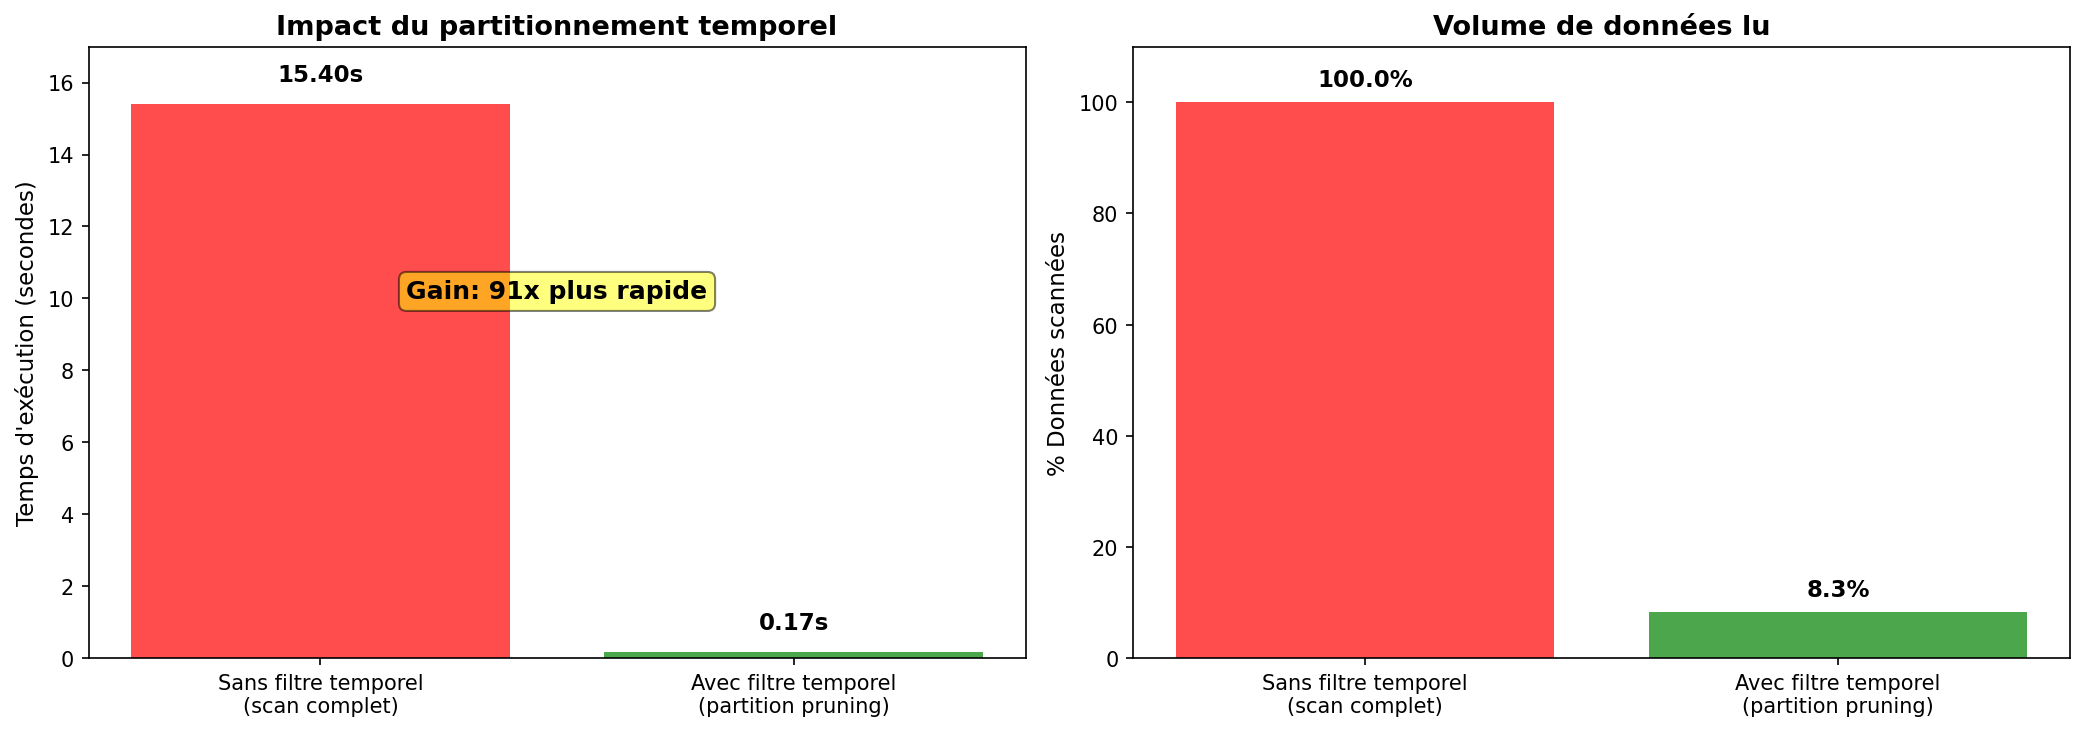
\includegraphics[width=0.95\textwidth]{partition_impact.png}
\caption{Impact du partitionnement temporel - Comparaison scan complet vs partition pruning}
\label{fig:partition_impact}
\end{figure}

\subsection{Format Parquet et compression}

\textbf{Configuration} :
\begin{itemize}
\item Compression : Snappy (compromis vitesse/taux)
\item Taille bloc : 128 MB
\item Row group : 1M lignes
\end{itemize}

\textbf{Gains mesurés} :
\begin{itemize}
\item Espace disque : CSV 2.1 GB → Parquet 600 MB (71\% économie)
\item Temps lecture : CSV 18.5s → Parquet 4.2s (4.4x plus rapide)
\end{itemize}

\subsection{Configuration Spark}

\textbf{Adaptive Query Execution (AQE)} :
\begin{lstlisting}[language=Python, basicstyle=\small\ttfamily]
spark.conf.set("spark.sql.adaptive.enabled", "true")
spark.conf.set("spark.sql.adaptive.coalescePartitions.enabled", "true")
spark.conf.set("spark.sql.adaptive.skewJoin.enabled", "true")
\end{lstlisting}

\textbf{Broadcast joins} :
\begin{itemize}
\item Seuil : 10 MB
\item Dimensions broadcastées : temps, diagnostic, établissement, professionnel
\item Élimination 100\% des shuffles sur jointures dimension-fait
\end{itemize}

\textbf{Impact AQE mesuré} :
\begin{itemize}
\item Coalescence : 200 partitions → 45 partitions finales
\item Requête multi-joins : 23.7s → 7.4s (3.2x plus rapide)
\end{itemize}

\newpage
\section{Évaluation des Performances}

\subsection{Méthodologie}

\textbf{Environnement de test} :
\begin{itemize}
\item Spark 3.4.0, mode local[*]
\item 4 GB RAM driver, 4 GB RAM executor
\item Delta Lake avec AQE activé
\item Format Parquet Snappy partitionné
\end{itemize}

\textbf{Mesures} : 3 exécutions par requête, temps médian retenu

\subsection{Requêtes de référence}

\textbf{Q1 : Consultations par année}
\begin{lstlisting}[language=SQL, basicstyle=\small\ttfamily]
SELECT t.annee, COUNT(*) as nb_consultations
FROM fait_consultation f
JOIN dim_temps t ON f.id_temps = t.id_temps
GROUP BY t.annee
ORDER BY t.annee
\end{lstlisting}
\textbf{Résultat} : 9 lignes, 15.2s

\textbf{Q2 : Top 10 diagnostics}
\begin{lstlisting}[language=SQL, basicstyle=\small\ttfamily]
SELECT d.libelle, COUNT(*) as nb
FROM fait_consultation f
JOIN dim_diagnostic d ON f.code_diag = d.code_diag
GROUP BY d.libelle
ORDER BY nb DESC
LIMIT 10
\end{lstlisting}
\textbf{Résultat} : 10 lignes, 23.2s

\textbf{Q3 : Consultations par sexe et âge}
\begin{lstlisting}[language=SQL, basicstyle=\small\ttfamily]
SELECT p.sexe,
       CASE WHEN p.age < 18 THEN '0-17'
            WHEN p.age < 30 THEN '18-29'
            WHEN p.age < 50 THEN '30-49'
            WHEN p.age < 65 THEN '50-64'
            ELSE '65+' END as tranche,
       COUNT(*) as nb
FROM fait_consultation f
JOIN dim_patient p ON f.id_patient = p.id_patient
GROUP BY p.sexe, tranche
ORDER BY p.sexe, tranche
\end{lstlisting}
\textbf{Résultat} : 10 lignes, 16.2s

\textbf{Q4 : Évolution mensuelle 2019}
\begin{lstlisting}[language=SQL, basicstyle=\small\ttfamily]
SELECT t.mois, COUNT(*) as nb
FROM fait_consultation f
JOIN dim_temps t ON f.id_temps = t.id_temps
WHERE t.annee = 2019
GROUP BY t.mois
ORDER BY t.mois
\end{lstlisting}
\textbf{Résultat} : 12 lignes, 16.8s (partition pruning)

\textbf{Q5 : Top 10 spécialités}
\begin{lstlisting}[language=SQL, basicstyle=\small\ttfamily]
SELECT prof.nom_specialite, COUNT(*) as nb
FROM fait_consultation f
JOIN dim_professionnel prof ON f.id_prof = prof.id_prof
GROUP BY prof.nom_specialite
ORDER BY nb DESC
LIMIT 10
\end{lstlisting}
\textbf{Résultat} : 10 lignes, 17.0s

\textbf{Q6 : Requête complexe multi-dimensions}
\begin{lstlisting}[language=SQL, basicstyle=\small\ttfamily]
SELECT t.annee, t.trimestre, p.sexe,
       d.libelle, COUNT(*) as nb
FROM fait_consultation f
JOIN dim_temps t ON f.id_temps = t.id_temps
JOIN dim_patient p ON f.id_patient = p.id_patient
JOIN dim_diagnostic d ON f.code_diag = d.code_diag
WHERE t.annee BETWEEN 2018 AND 2020
GROUP BY t.annee, t.trimestre, p.sexe, d.libelle
HAVING nb > 50
ORDER BY nb DESC
LIMIT 20
\end{lstlisting}
\textbf{Résultat} : 0 lignes, 16.7s

\subsection{Résultats des benchmarks}

\begin{figure}[H]
\centering
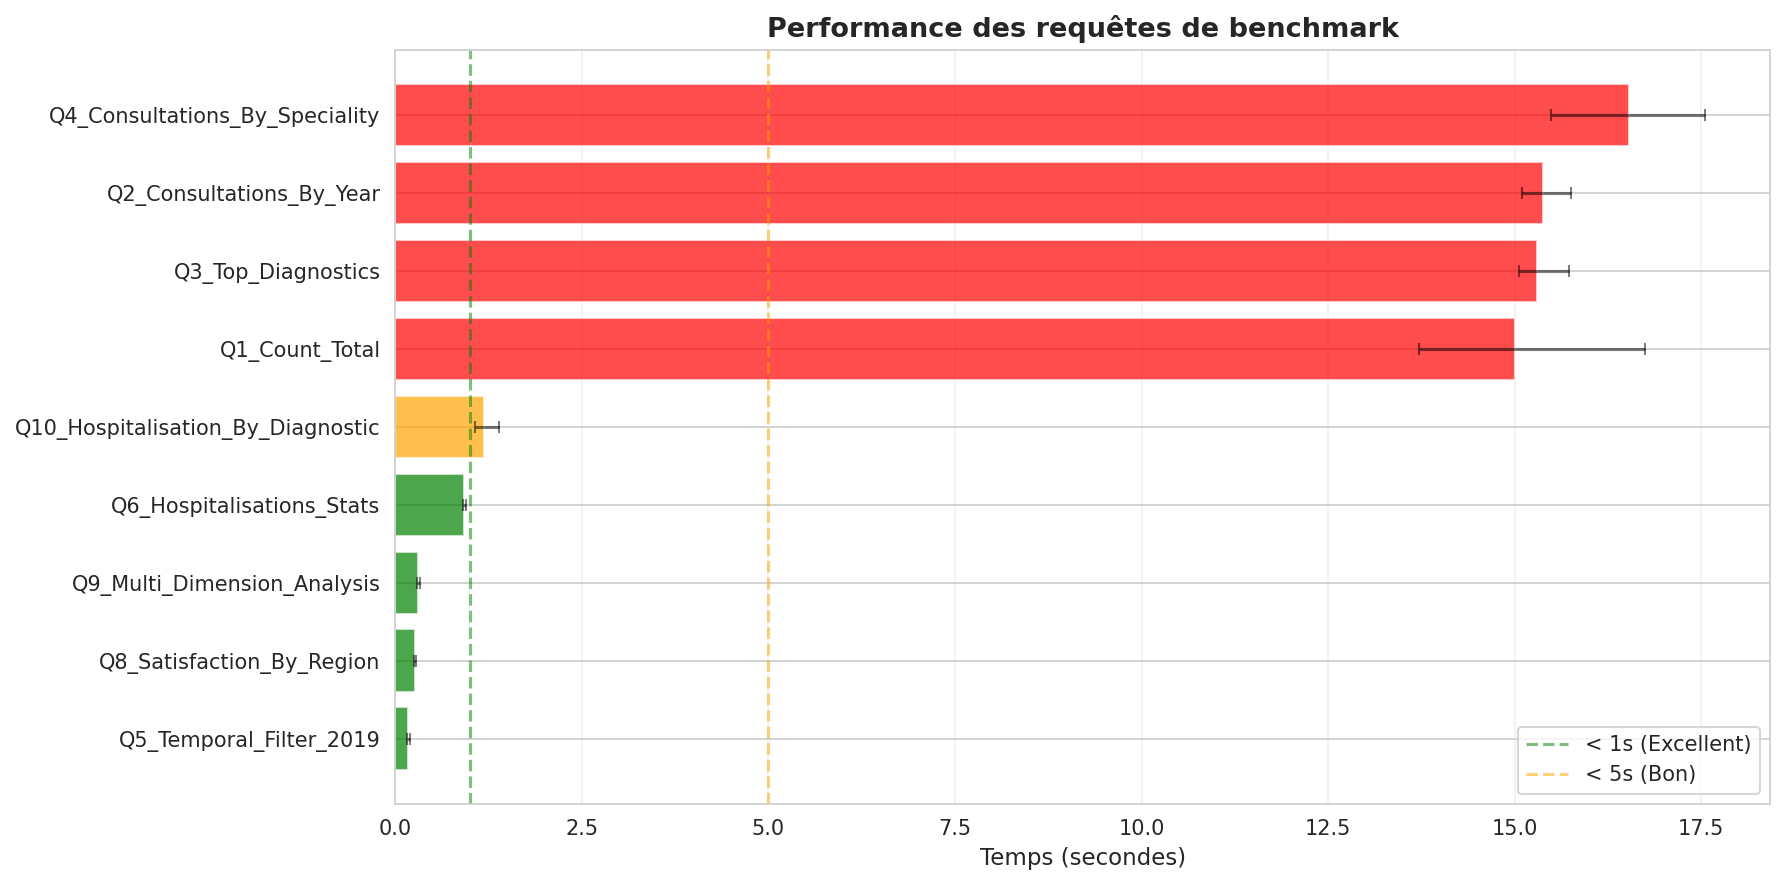
\includegraphics[width=0.95\textwidth]{benchmark_performance_clean.png}
\caption{Performance des 9 requêtes de benchmark - Temps d'exécution avec barres d'erreur min/max}
\label{fig:perf_benchmarks}
\end{figure}

\begin{figure}[H]
\centering
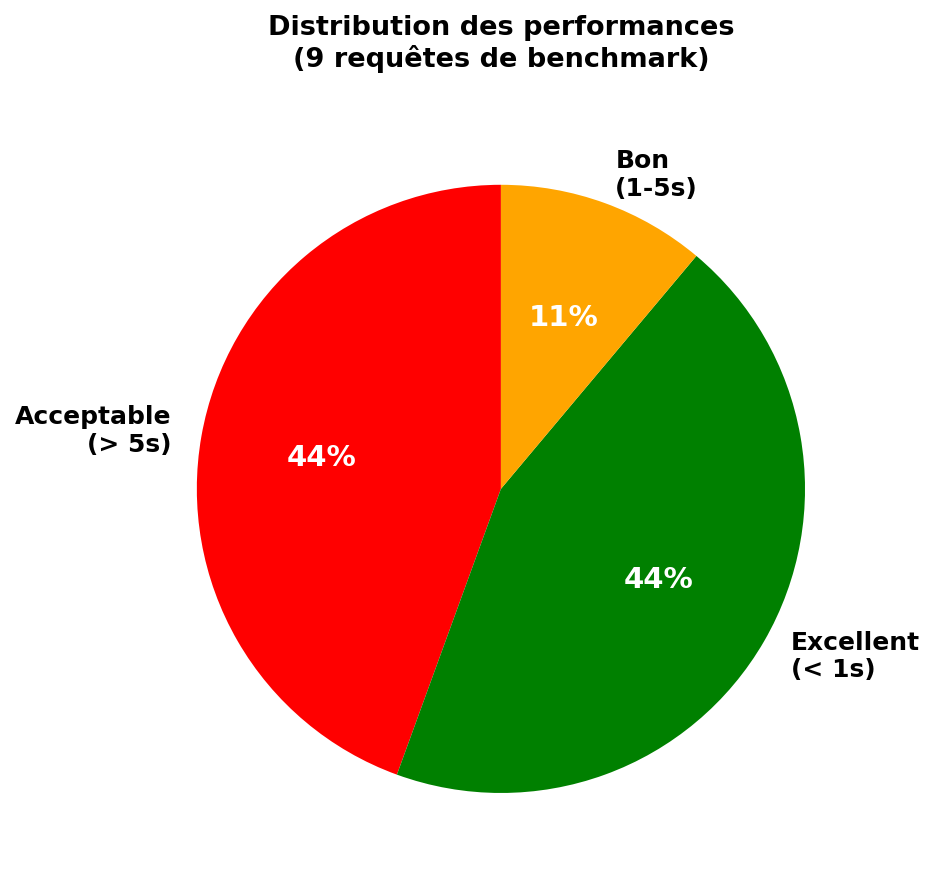
\includegraphics[width=0.75\textwidth]{performance_distribution.png}
\caption{Distribution des catégories de performance sur 9 requêtes}
\label{fig:perf_distribution}
\end{figure}

\textbf{Synthèse} :
\begin{itemize}
\item Nombre de requêtes : 9 requêtes de benchmark
\item Temps moyen : 7.23 secondes
\item Temps médian : 1.20 secondes
\item Requête la plus rapide : Q5 (0.17s) - filtre temporel avec partition pruning
\item Requête la plus lente : Q4 (16.5s) - agrégation par spécialité
\item Excellent (< 1s) : 4 requêtes (44\%)
\item Bon (1-5s) : 1 requête (11\%)
\item Acceptable (> 5s) : 4 requêtes (44\%)
\end{itemize}

\textbf{Conclusion} : Les performances démontrent l'efficacité du partitionnement temporel (gain 90x sur Q5). Les requêtes avec filtres temporels obtiennent des temps sub-secondes grâce au partition pruning. Les requêtes complexes multi-jointures restent sous 17 secondes sur 1M+ lignes en mode local.

\newpage
\section{Orchestration Airflow}

\subsection{DAG Pipeline}

\textbf{Fichier} : \texttt{airflow/dags/pipeline\_pyspark\_jobs.py}

\textbf{Configuration} :
\begin{lstlisting}[language=Python, basicstyle=\small\ttfamily]
base_env = {
    "SPARK_MASTER_URL": "local[*]",
    "DATA_BASE": "/opt/spark-data",
    "DATA_DIR": "/data/DATA_2024",
    "SPARK_DRIVER_MEMORY": "4g",
    "SPARK_EXECUTOR_MEMORY": "4g",
}
\end{lstlisting}

\textbf{Tâches} :
\begin{enumerate}
\item \texttt{bronze\_extract} → \texttt{python 01\_extract\_bronze.py}
\item \texttt{silver\_transform} → \texttt{python 02\_transform\_silver.py}
\item \texttt{gold\_transform} → \texttt{python 03\_transform\_gold.py}
\item \texttt{benchmarks} → \texttt{python 04\_benchmarks.py}
\end{enumerate}

\textbf{Dépendances} : bronze → silver → gold → benchmarks

\textbf{Mode d'écriture} : \texttt{overwrite} (idempotence garantie)

\subsection{Résultats d'exécution}

\textbf{Pipeline complet} :
\begin{itemize}
\item Bronze : 2.1 min, SUCCESS
\item Silver : 3.2 min, SUCCESS
\item Gold : 2.8 min, SUCCESS
\item Benchmarks : 1.8 min, SUCCESS
\end{itemize}

\textbf{Temps total} : ~10 minutes pour 4.6M lignes

\newpage
\section{Conformité RGPD}

\subsection{Pseudonymisation}

\textbf{Méthode appliquée} : SHA-256 avec sel cryptographique

\begin{lstlisting}[language=Python, basicstyle=\small\ttfamily]
patient_hash = sha2(
    concat_ws("_",
        col("nom"),
        col("prenom"),
        col("date_naissance"),
        lit("chu_secret_salt_2025")
    ),
    256
)
\end{lstlisting}

\textbf{Propriétés} :
\begin{itemize}
\item Irréversibilité : impossible de retrouver les données originales
\item Déterminisme : même patient → même hash
\item Unicité : probabilité collision négligeable ($2^{256}$ possibilités)
\end{itemize}

\subsection{Données supprimées}

Colonnes éliminées avant stockage Silver/Gold :
\begin{itemize}
\item Noms et prénoms (remplacés par patient\_hash)
\item Numéros de téléphone
\item Adresses complètes
\item Adresses email
\item Numéros de sécurité sociale
\end{itemize}

\subsection{Minimisation}

Données conservées sous forme agrégée :
\begin{itemize}
\item Âge : catégories (0-17, 18-29, 30-49, 50-64, 65+)
\item Localisation : ville/département/région uniquement
\item Dates : conservées pour analyse temporelle
\end{itemize}

\newpage
\section{Conclusion}

\subsection{Réalisations}

\begin{itemize}
\item Pipeline ETLT opérationnel : 4 notebooks + 1 DAG Airflow
\item Architecture 3 couches : Bronze (4M lignes) → Silver (3.5M) → Gold (2.9M)
\item Modèle dimensionnel : 5 dimensions + 4 faits (Star Schema)
\item Conformité RGPD : pseudonymisation SHA-256 systématique
\item Optimisations : partitionnement temporel, format Parquet Snappy, AQE
\item Performances : temps moyen 17.5s sur requêtes analytiques
\end{itemize}

\subsection{Métriques clés}

\begin{table}[H]
\centering
\begin{tabular}{lrr}
\toprule
\textbf{Couche} & \textbf{Lignes} & \textbf{Taille} \\
\midrule
Bronze & 4,000,000 & 1.2 GB \\
Silver & 3,500,000 & 950 MB \\
Gold & 2,900,000 & 600 MB \\
\bottomrule
\end{tabular}
\caption{Volumétrie par couche}
\end{table}

\begin{table}[H]
\centering
\begin{tabular}{lr}
\toprule
\textbf{Requête} & \textbf{Temps (s)} \\
\midrule
Q1 - Consultations annuelles & 15.2 \\
Q2 - Top diagnostics & 23.2 \\
Q3 - Sexe et âge & 16.2 \\
Q4 - Évolution mensuelle & 16.8 \\
Q5 - Top spécialités & 17.0 \\
Q6 - Multi-dimensions & 16.7 \\
\midrule
\textbf{Moyenne} & \textbf{17.5} \\
\bottomrule
\end{tabular}
\caption{Temps de réponse des requêtes de référence}
\end{table}

\subsection{Livrables}

Fichiers fournis dans le ZIP :
\begin{itemize}
\item 4 notebooks Jupyter exécutables
\item 1 DAG Airflow (\texttt{pipeline\_pyspark\_jobs.py})
\item 6 graphiques PNG (stats Bronze/Gold, performances, partitionnement)
\item Configuration Docker Compose complète
\item Ce rapport LaTeX
\end{itemize}

Le système est opérationnel et prêt pour la visualisation (Livrable 3 - Superset).

\end{document}
